% !TEX TS-program = pdflatex
% !TEX encoding = UTF-8 Unicode

% This is a simple template for a LaTeX document using the "article" class.
% See "book", "report", "letter" for other types of document.

\documentclass[11pt,titlepage]{article} % use larger type; default would be 10pt

\usepackage[utf8]{inputenc} % set input encoding (not needed with XeLaTeX)

%%% Examples of Article customizations
% These packages are optional, depending whether you want the features they provide.
% See the LaTeX Companion or other references for full information.

%%% PAGE DIMENSIONS
\usepackage{geometry} % to change the page dimensions
\geometry{a4paper} % or letterpaper (US) or a5paper or....
\geometry{margin=2cm} % for example, change the margins to 2 inches all round
\geometry{portrait} % set up the page for landscape
%   read geometry.pdf for detailed page layout information

\usepackage{graphicx} % support the \includegraphics command and options
\usepackage{float}
\usepackage[parfill]{parskip} % Activate to begin paragraphs with an empty line rather than an indent

%%% PACKAGES
%\usepackage{booktabs} % for much better looking tables
%\usepackage{array} % for better arrays (eg matrices) in maths
%\usepackage{paralist} % very flexible & customisable lists (eg. enumerate/itemize, etc.)
\usepackage{verbatim} % adds environment for commenting out blocks of text & for better verbatim
%\usepackage{subfig} % make it possible to include more than one captioned figure/table in a single float
% These packages are all incorporated in the memoir class to one degree or another...
%\usepackage{glossaries} %for the glossary

%%% HEADERS & FOOTERS
%\usepackage{fancyhdr} % This should be set AFTER setting up the page geometry
%\pagestyle{fancy} % options: empty , plain , fancy
%\renewcommand{\headrulewidth}{0pt} % customise the layout...
%\lhead{}\chead{}\rhead{}
%\lfoot{}\cfoot{\thepage}\rfoot{}

%%% SECTION TITLE APPEARANCE
%\usepackage{sectsty}
%\allsectionsfont{\sffamily\mdseries\upshape} % (See the fntguide.pdf for font help)
% (This matches ConTeXt defaults)

%%% ToC (table of contents) APPEARANCE
%\usepackage[nottoc,notlof,notlot]{tocbibind} % Put the bibliography in the ToC
%\usepackage[titles,subfigure]{tocloft} % Alter the style of the Table of Contents
%\renewcommand{\cftsecfont}{\rmfamily\mdseries\upshape}
%\renewcommand{\cftsecpagefont}{\rmfamily\mdseries\upshape} % No bold!

%%% END Article customizations

%%% The "real" document content comes below...

%%% Maketitle metadata
\newcommand{\horrule}[1]{\rule{\linewidth}{#1}} 	% Horizontal rule

\title{
		\normalfont \normalsize \textsc{Client Name: DVT} \\
		\normalfont \normalsize \textsc{Project Name: KinderFinder} \\ [25pt]
		\horrule{0.5pt} \\[0.4cm]
		\huge This is the title of the template report \\
		\horrule{2pt} \\[0.5cm]
}
\author{\begin{tabular}{rl}
	\texttt{Team Name:} & \texttt{MAU Technologies} \\[0.5cm]
	Uteshlen Nadesan & 28163304 \\
	Michael Johnston & 12053300 \\
	Po-Han Chiu & 11063612
\end{tabular}
	\\ \\ \texttt{https://github.com/MrBean355/KinderFinder.git}
	\\ \\ \texttt{Version: 0.0}}
\date{23 May 2014}  
% Activate to display a given date or no date (if empty),
         % otherwise the current date is printed -------

%%% Begin document
\begin{document}
\maketitle
\tableofcontents
\newpage

\section{Functional requirements and application design}

\subsection{Introduction}
This section discusses the functional requirements for the KinderFinder System, this introduces the core domain concepts and relationships between these concepts.

The requirement is to create a system, that will through the use of RFID technology in wristbands and matching readers / receivers, be able to track children throughout a restaurant or designated area. This information needs to be fed to an API on a server that will push information to the relevant devices (mobile) to inform parents of the children's whereabouts within the designated area.
\subsection{Required functionality}

	\subsubsection{Web Administration}
The Web administration must:
\begin{itemize}
\item Be used to allow installers of the system to set-up restaurants and their layouts (using 
maps). 
\item Enable  restaurants to link  wristbands  to  a Patron’s mobile application, or assigned 
electronic tracking device (device not in scope).
\item Enable restaurants to clear and unlink wristbands from devices and patrons’ mobile 
apps.
\item Allow access to basic reporting will also be done through the Web Administration.
\end{itemize}

	\subsubsection{Mobile Application}
The mobile implementation must:
\begin{itemize}
\item Allow for users to view a map (divided into zones) of the restaurant.
\item Overlay all the wristbands registered on the app user’s name on the map to show 
where they are (some patrons might have multiple children to track).
\item Allow  for  setting  up  of  alarms  and  notifications  based  on  movement  of  tracked 
wristbands. 
\item Allow for a user to select a restaurant, and a restaurant branch in order to get the 
map for the set-up. 
\item Enable the user to link the wristband to their  mobile application
\end{itemize}

	\subsubsection{Web API}
	The  system  must  have  a  central  web  based  API  that  concerns  itself  with  gathering 
information and supplying information from the system. This API will be used by:
\begin{itemize}
\item Mobile Application
\item Web Administration
\item A Service, if needed, that can push information to devices
\end{itemize}
Therefore this API must be loosely coupled from any implementation using it ,  as it needs to 
be re-used for multiple implementations, and possible future applications / implementations.

	\subsubsection{Basic Reporting}
	\begin{itemize}
	\item Facility usage  (zone based) by children. This will enable a restaurant to see statistics 
on which areas are most popular for children.
\item Usage statistic of mobile app users that could possibly enable restaurant chains to 
implement a loyalty program.
\item Health reports, reports that will indicate the health of the hardware being used. This should pick up trends that are impossible with the restaurant layout.
\end{itemize}	

	\subsubsection{Embedded Hardware and prototyping}
Physical hardware devices used in this project includes:
\begin{itemize}
\item Receiver/Reader prototype
	\begin{itemize}
	\item These  are  devices  that  are  placed  at  predetermined  locations  within  the 
		designated area where tracking will occur in order to pick up wristbands and their relative signal strengths.  				These devices will use wireless communication will to communicate this information to an access point with 					internet access
	\end{itemize}	
\item Wristband prototype
	\begin{itemize}
		\item These  can  be  active  or  passive  RFID  tags,  or 					wireless transponders/transceivers. They will be used to 			communicate its existence in range of a receiver/reader 				and its signal strength (RS SI)
	\end{itemize}
	
\item Electronic tracking device	
\begin{itemize}
\item This device, when developed, will be a piece of hardware the patron can put on their table with LED’s representing zones on the restaurant map. However, for this project it is not of concern, however, it should be kept in mind during implementation for future implementation and programming.
\end{itemize}	
\end{itemize}
	
\subsection{Use case prioritization}
	Here we are considering a simple 3 level use case prioritization, with critical functionality (a use case or function that is absolutely essential), important functionality (if a system would still be basically functioning but still less than the client specification) and, nice-to-haves (added functionality that the client would not consider core but would add to the presentation of the project).
	
	\subsubsection{Critical}
\begin{itemize}
\item Database - A database containing all relevant information about users, restaurants/stores and the RFID bands and readers.
\item Web Administration - This requirement is essential. It allows the proper operation of the program, as web administration allows installation of this system.
\item Mobile Administration - This is the part of the system the end-user will be able to use. This is one of two main interfaces with the end-user.
\item WEB API - The Web API is the core of the system, it provides functionality to the client browsers and the mobile applications.
\end{itemize}

	\subsubsection{Important}
\begin{itemize}
\item Basic Reporting - The reporting portion of the system is useful for logging and statistics. Even though the data gathered will be useful, the core system will still function. (Not to say this will not be done.)
\end{itemize}

	\subsubsection{Nice-To-Have}
\begin{itemize}
\item Embedded Hardware and Prototyping - This is the RFID wrist bands and RFID readers. Mock data will be used for testing and implementation, after which, our team will focus on the hardware prototyping and testing.
\end{itemize}


\subsection{Use case/Services contracts}
	\subsubsection{Use Case Login}
\begin{figure}[H]
\centering
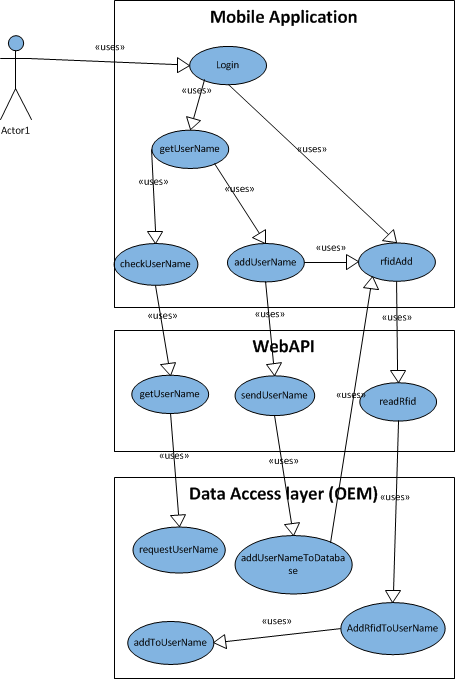
\includegraphics[scale = 0.8]{UseCaseLogin.png}
\caption{Use Case Diagram - Login}
\end{figure}
\begin{itemize}
\item Pre-Conditions - There are no pre-conditions for this use case besides having the application on the user's mobile.
\item Post-Conditions - After the user has logged on and added the required RFID tag to their profile, the profile should remain active and requesting updates from the WEB API.
\end{itemize}
	

%\subsection{Process specifications}

\subsection{Domain Objects}

\subsubsection{Data Base}
A data base diagram in the form of an ERD has been drafted and shown below. Because we do not know what extra might be needed during development, we will keep evolving the data base to meet our required functionality. 

\begin{figure}[H]
\centering
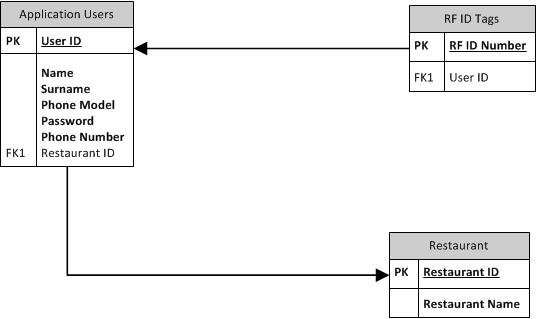
\includegraphics[scale=1]{ERDKinderFinderDatabase.jpg} 
\caption{ERD Data Base}
\end{figure}


\newpage













\appendix
\section{\\Title of Appendix A} \label{App:AppendixA}
% the \\ insures the section title is centered below the phrase: AppendixA

Text of Appendix A is Here

\newpage
\section{\\Title of Appendix B} \label{App:AppendixB}
% the \\ insures the section title is centered below the phrase: Appendix B

Text of Appendix B is Here

\newpage
\begin{thebibliography}{10}

\bibitem{First Reference}

\end{thebibliography}
%\printglossary
\end{document}
